\chapter{Конструкторский раздел}
    
В данном разделе будет описан алгоритм предобработки данных и алгоритм работы ПО, осуществляющего решение задачи регрессии.

\section{Алгоритм предобработки данных}
\begin{enumerate}
    \item Инициализируется пустой словарь, который будет использоваться для хранения соответствия между уникальными значениями и их кодами.
    \item Поступает массив значений, который нужно закодировать.
    \item Сначала необходимо пройти по всем значениям во входном массиве и вычислить уникальные значения.
    \item Далее каждому уникальному значению присваивается уникальный код, начиная с 0 и увеличиваясь на 1 для каждого нового уникального значения.
    \item Полученные соответствия между уникальными значениями и их кодами сохраняются в словаре.
    \item Затем каждый элемента во входном массиве значений заменяется на соответствующий ему код из словаря.
    \item В итоге возвращается массив закодированных числовых меток, где каждое значение заменено на соответствующий ему код.
    \item Этот закодированный массив может быть использован для обучения моделей машинного обучения, которые требуют числовых данных в качестве входа.
\end{enumerate}
Алгоритм предобработки данных приведён на рисунке \ref{fig:prep}.
\newpage
\begin{figure}[h!]
	\centering
	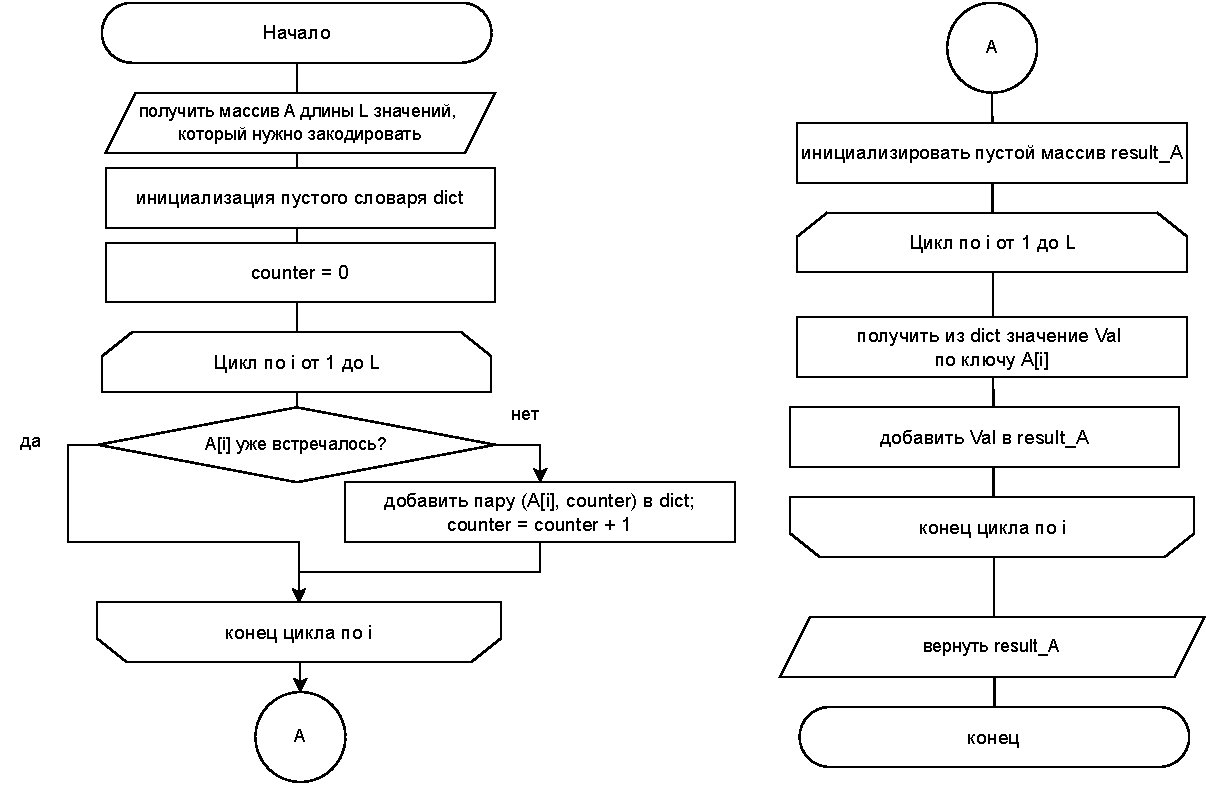
\includegraphics[width = \linewidth]{img/prep.pdf}
	\caption{Алгоритм предобработки данных}
	\label{fig:prep}
\end{figure}

\section{Алгоритм работы ПО}
Основной алгоритм работы ПО состоит из 3 основных шагов: 
\begin{itemize}
    \item подготовки данных -- преобразование всех нечисловых данные в числовой вид с помощью алгоритма, описанного в предыдущем пункте;
    \item обучение модели градиентного бустинга на обучающей выборке, полученной из исходного набора данных;
    \item вычисление значения метрики MAPE на тестовой выборке, полученной из исходного набора данных так, что она не пересекается с обучающей выборкой. 
\end{itemize}

\newpage
Алгоритм работы ПО приведён на рисунке \ref{fig:common}.
\begin{figure}[h!]
	\centering
	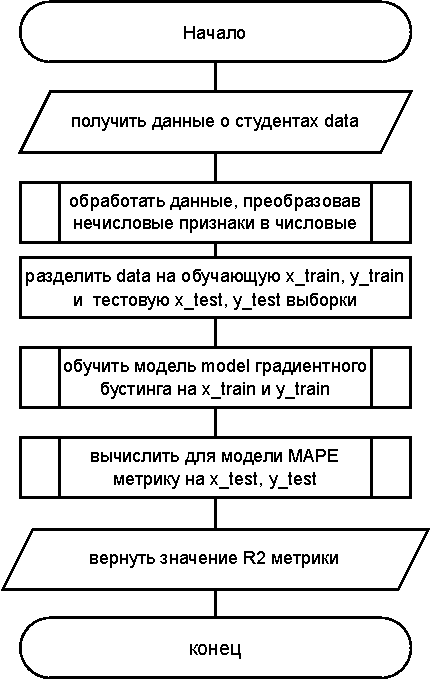
\includegraphics[scale = 1]{img/base.pdf}
	\caption{Алгоритм работы ПО}
	\label{fig:common}
\end{figure}




\section*{Вывод}
\addcontentsline{toc}{section}{Вывод}

В данном разделе был описан алгоритм предобработки данных и алгоритм работы ПО, осуществляющего решение задачи регрессии.

